\documentclass[11pt]{article}
\usepackage{authblk}
\usepackage{hyperref}
\usepackage{graphicx}
\graphicspath{ {./} }

\usepackage[square,numbers]{natbib}
\bibliographystyle{abbrvnat}

\newcommand{\numpy}{{\tt numpy}}    % tt font for numpy

\topmargin -.5in
\textheight 9in
\oddsidemargin -.25in
\evensidemargin -.25in
\textwidth 7in

\begin{document}

% ========== Edit your name here
\author[1]{Prof Emmanouil Tranos}
\affil[1]{School of Geographical Sciences, University of Bristol and The Alan Turing Institute}

\title{Digital economy in the UK: a multi-scalar story of the diffusion of web technologies}
\maketitle

\begin{center}
\href{mailto:e.tranos@bristol.ac.uk}{e.tranos@bristol.ac.uk},
\href{https://etranos.info/}{etranos.info}
%\href{https://twitter.com/EmmanouilTranos}{@EmmanouilTranos} \&
%\href{https://www.linkedin.com/in/emmanouil-tranos-42947812a/}{LinkedIn}
\end{center}

\medskip

This paper maps and models the participation in the digital economy and its evolution in the UK over space and time. Most of the existing economic geography literature which dealt with the spatiality of the internet employed supply-side measures, such as infrastructural capacity, in order to understand the geography of the digital economy and its potential spatial economic effects. Useful as these approaches might have been, they cannot capture the micro-processes and the characteristics of the individual online behaviour. Using large volumes of archived and geolocated web content, this paper models the diffusion of web technologies over space and time in the UK. Instead of using metrics capturing the passive engagement with digital technologies, for instance internet subscription metrics, this paper targets the active engagement with the digital as reflected in website creation. 

Importantly, the data and geolocation strategy allow to capture these processes at small spatial scales. This level of granularity differentiate this paper with previous approaches in the literature, which were only able to capture technological adoption at more coarse level. Thus, this paper tests how well established theoretical approaches regarding the diffusion of new technologies are still applicable when the focus is on local scales. Although we know that spatial contagion and urban hierarchies are key drivers of technological diffusion, such theoretical concepts have not been tested at small geographical scales. Apart from an empirical interest, understanding such processes at small scales can support designing strategies for the adoption of new technologies and the development of relevant infrastructure. 

The paper begins with simple analytical tools which reveal the scale-free character of the 'S curve' that defines the diffusion of new technologies and innovations. Indeed, such an 'S curve' describes the adoption of web technologies across scales and even at the level of local authorities in the UK (Figure \ref{fig:s}). Then, the paper continues with exploratory approaches, which signal the spatial dependence of the diffusion on web technologies. All the above provide useful insights for the last section, when the paper employs state of the art machine learning techniques to predict the diffusion of web technologies over space. Specifically, Random Forest models are trained at two different scales: local authorities (c. 400 in the UK) and census output areas (c. 230,000). The models are firstly trained and tested in all data using space and time sensitive \emph{k}-folds. This modelling exercise highlights the importance of the key spatial predictors as described in the literature in predicting technological diffusion. Then, these model are trained for each UK region separately and tested iteratively to all other regions in order obtain an understanding of how differently these spatial drivers affect the diffusion of web technologies across different places (Figures \ref{fig:la} and \ref{fig:oa}). In other words, this modelling strategy reveals how different or not UK regions have been in terms of the adoption of web technologies across scales. The granularity of the data used here allows to expose spatial differences that otherwise would have gone unnoticed. The results of the analysis depict diffusion mechanisms which can be very useful in understanding the evolutionary patterns of the adoption of other newer technologies.

\begin{figure}[h]
    \centering
    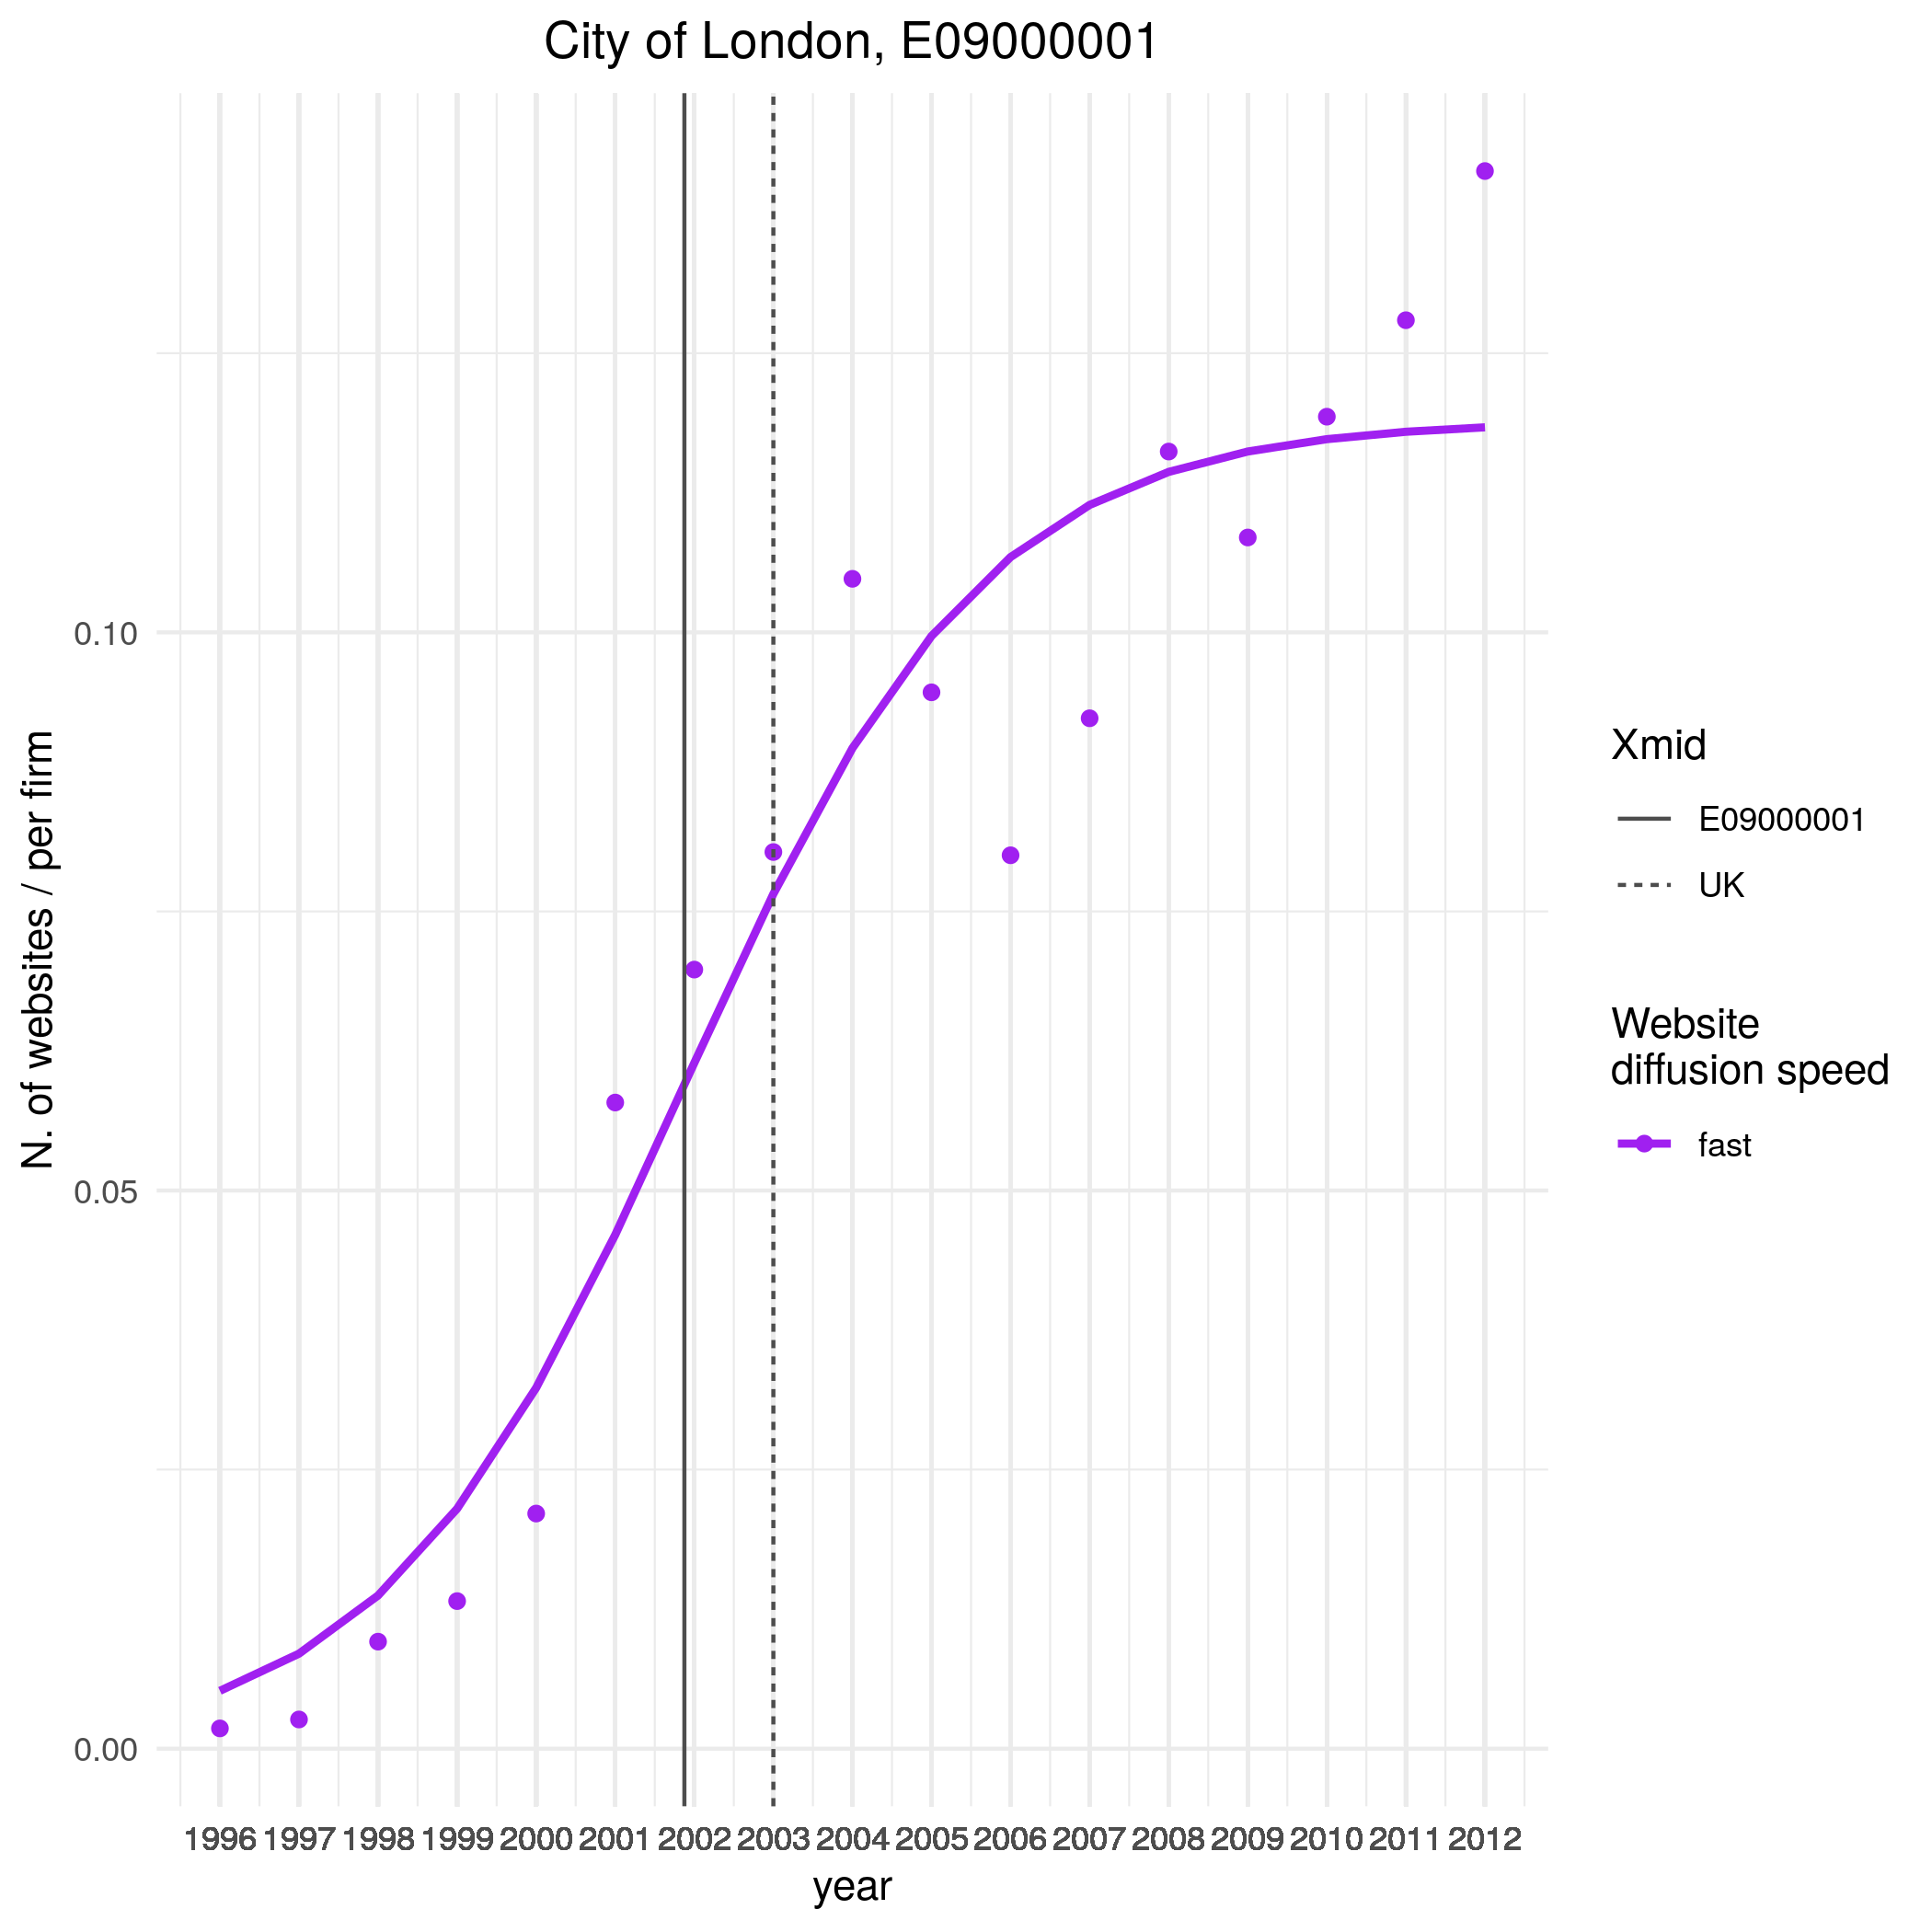
\includegraphics[width=0.75\textwidth]{lad_E09000001}
    \caption{Example of an S-curve for a local authority}
    \label{fig:s}
\end{figure}

\begin{figure}[h]
    \centering
    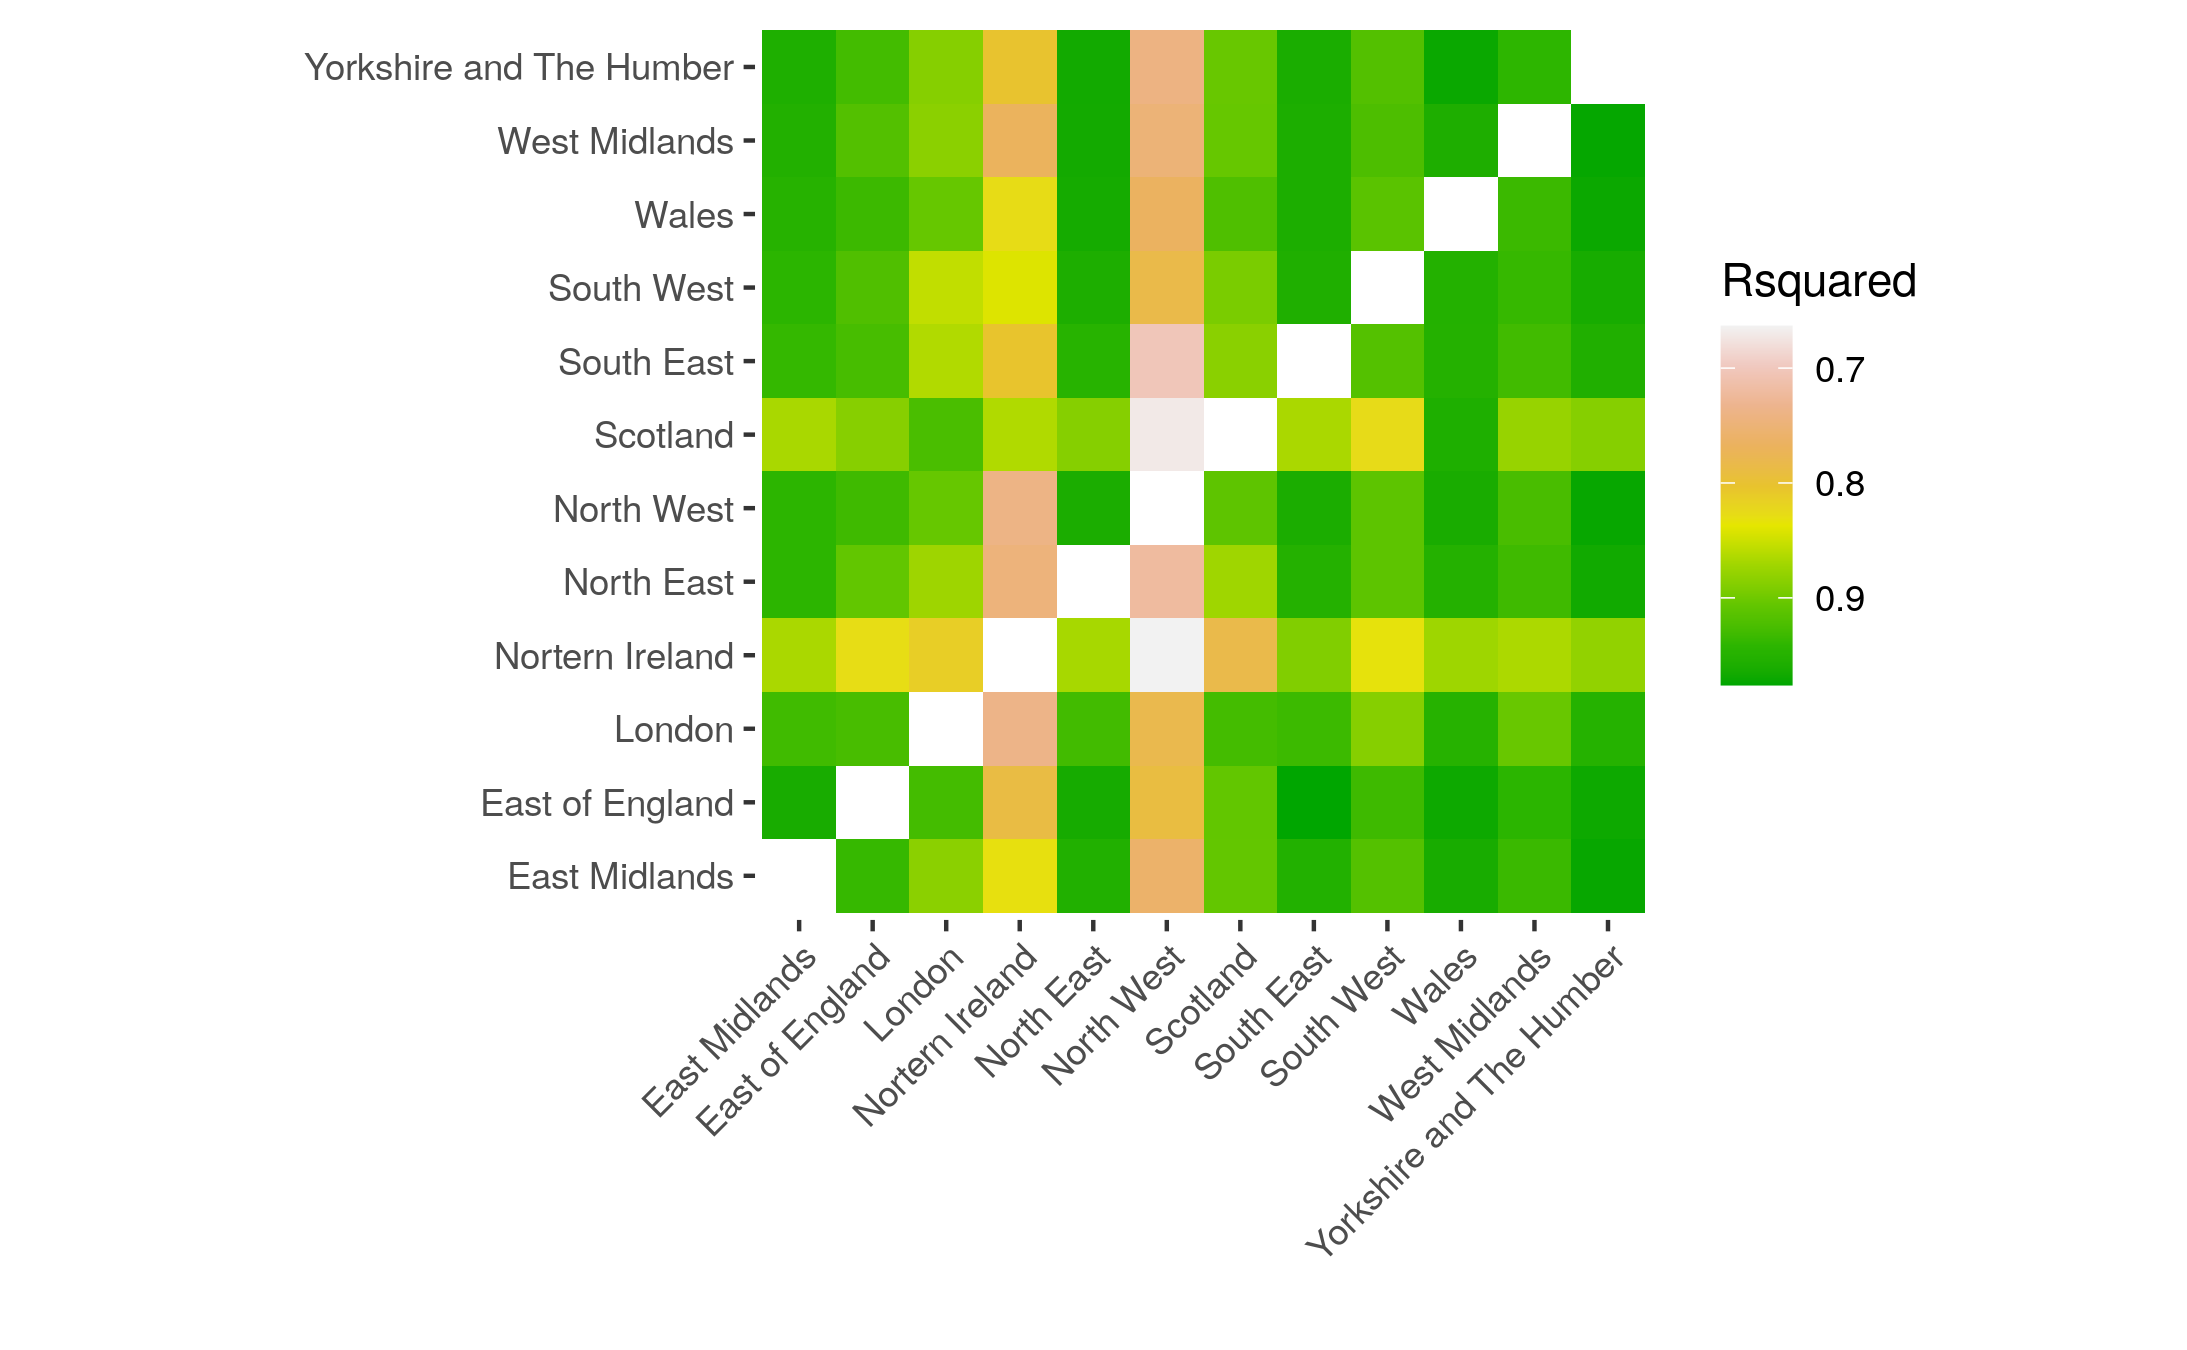
\includegraphics[width=0.9\textwidth]{heatmap_LA}
    \caption{Regional similarities based on cross-region training/predictions at the Local Authority level}
    \label{fig:la}
\end{figure}

\begin{figure}[h]
    \centering
    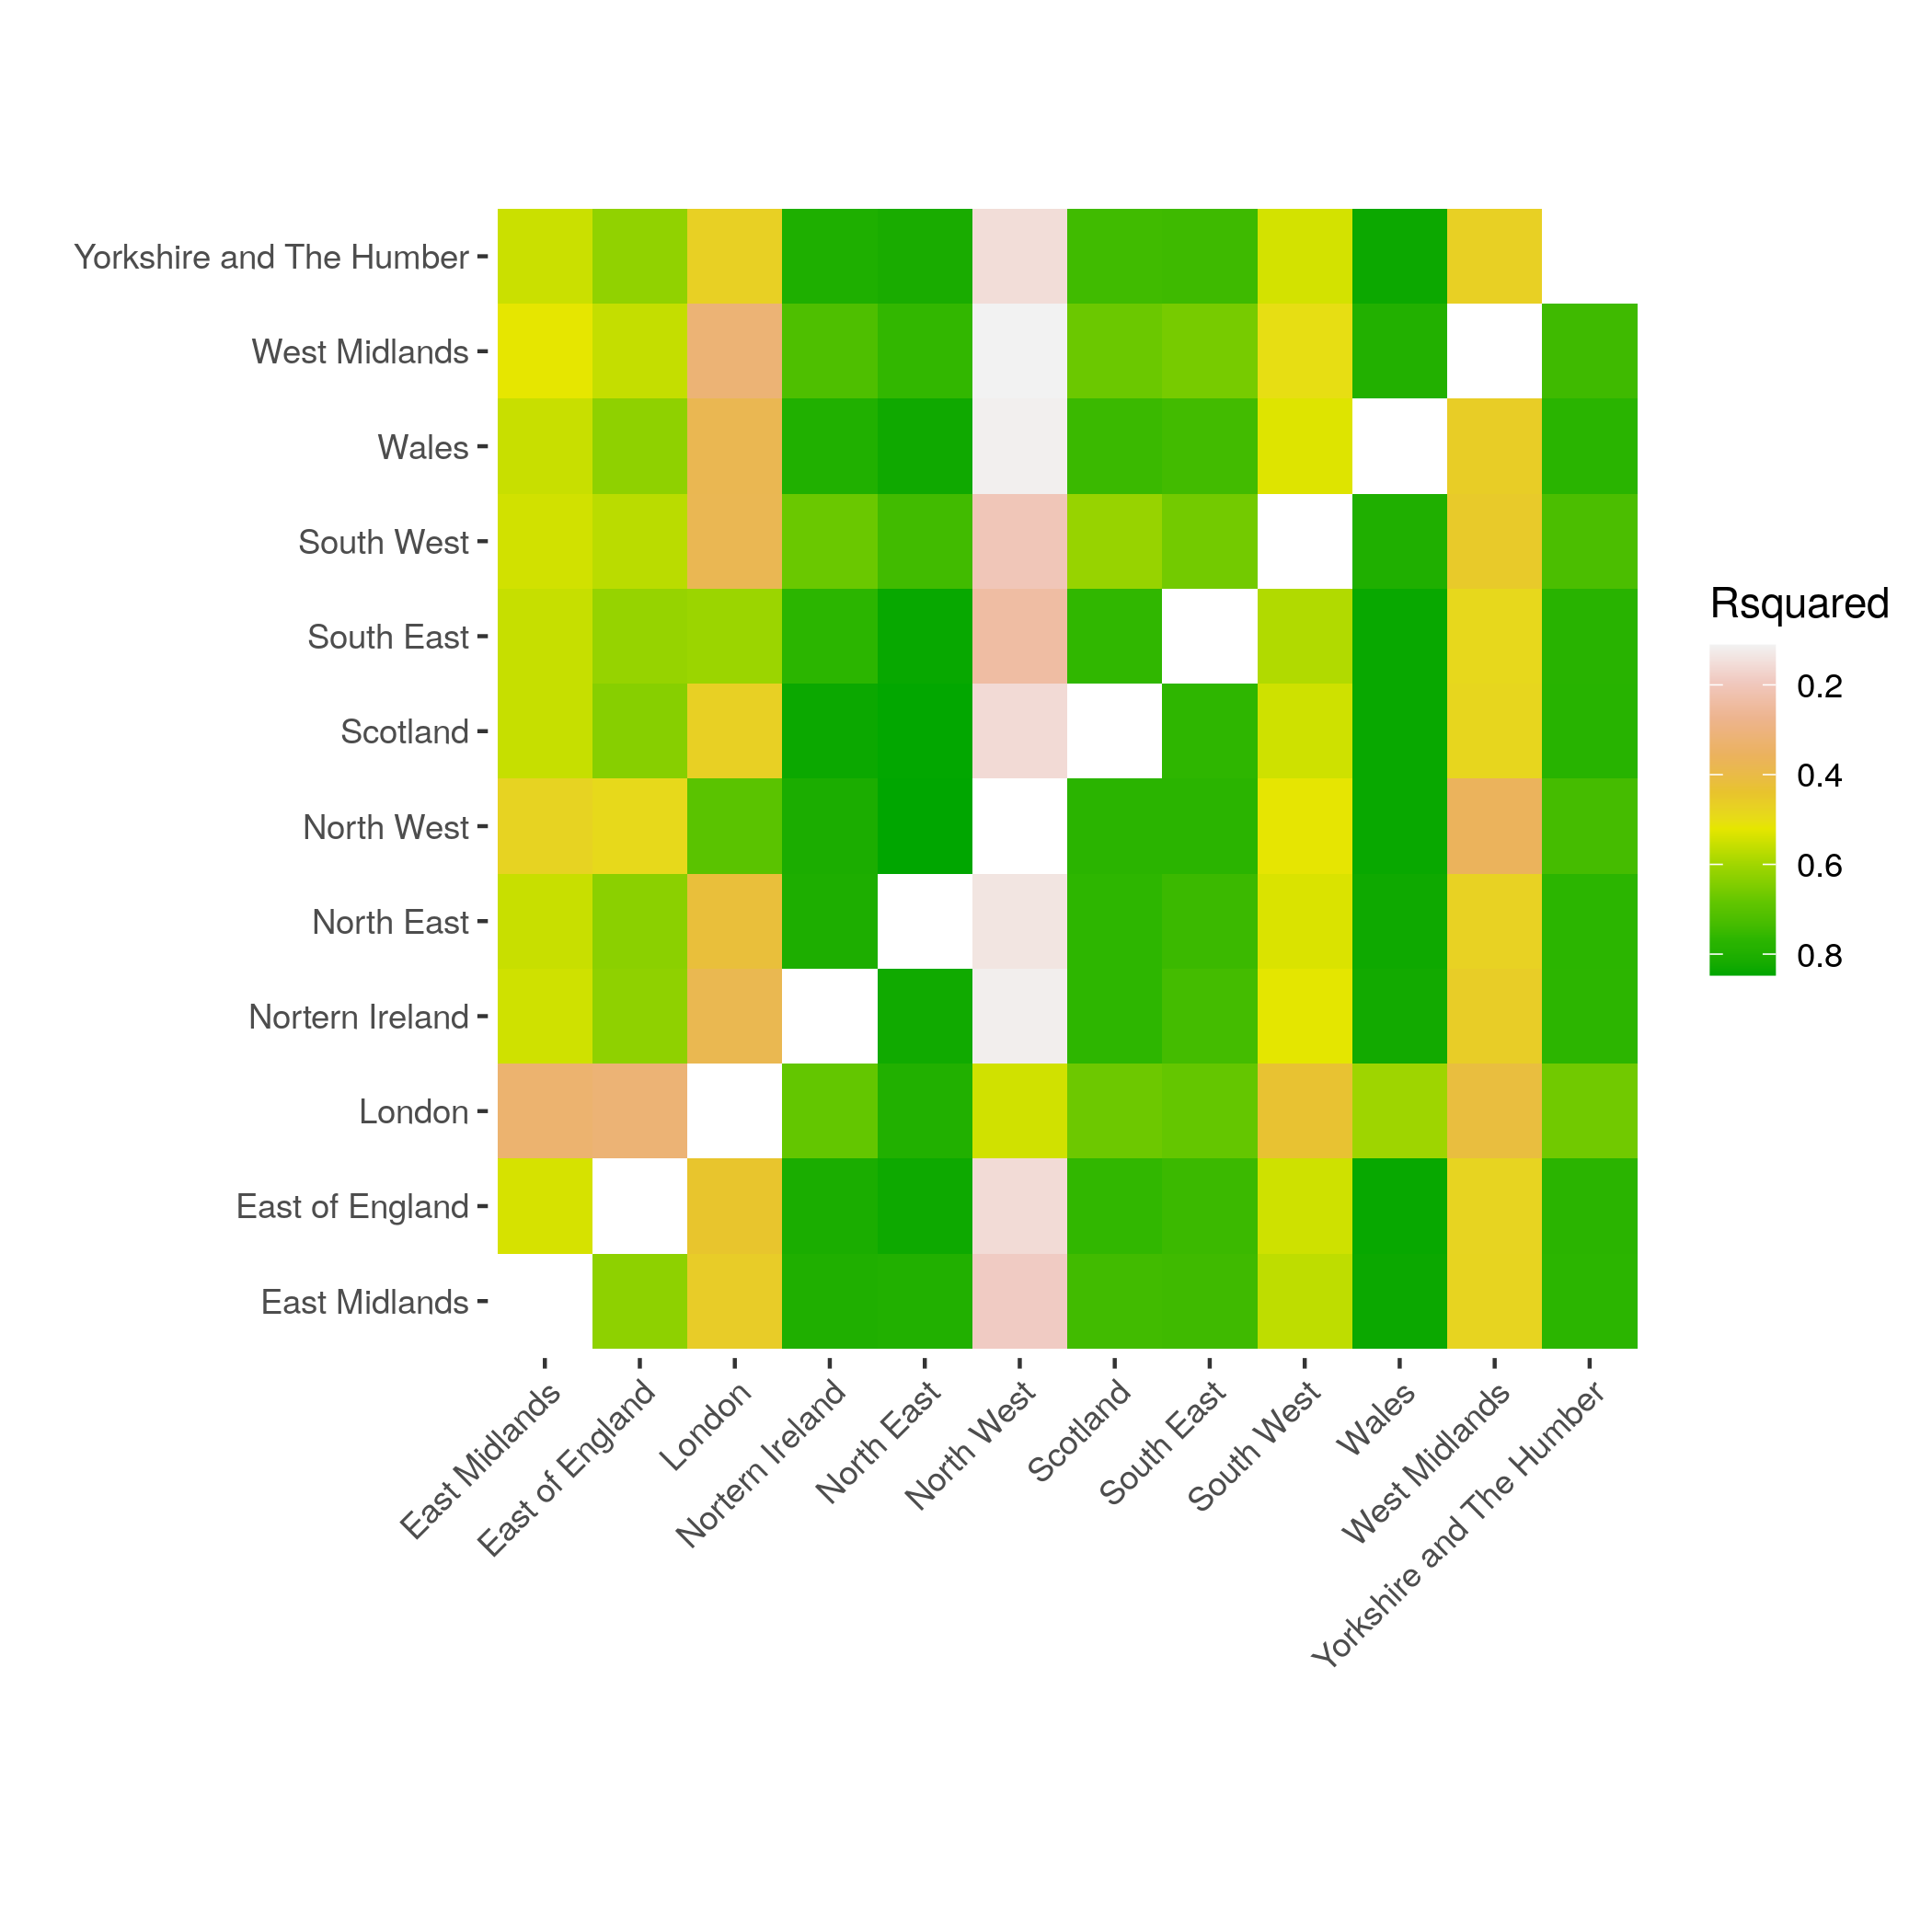
\includegraphics[width=0.75\textwidth]{heatmap_OA}
    \caption{Regional similarities based on cross-region training/predictions at the Local Authority level}
    \label{fig:oa}
\end{figure}

%\newpage
%\bibliography{bibliography}

\end{document}
\grid
\grid
